```
\documentclass[a4paper,10pt]{ctexart}

\setlength{\parindent}{0pt}% 设计全局无缩进
\usepackage{dirtree}
\usepackage{listings}
\usepackage{pythonhighlight}
\usepackage{ulem}%定义下划线
\usepackage{tikz}
\usetikzlibrary{mindmap}
\usetikzlibrary{positioning}

\begin{document}

\title{Python学习笔记}
\author{郑念祖}
\date{2017/3/15}
\maketitle

\section{基础知识}

\subsection{字符串 }
\begin{itemize}
  \item  \' ------->转义字符\ 单引号
  \item 双\ ------->对自身进行转义
  \item r'原始字符串'------->对所有反斜杠加入转义字符
  \item ‘‘‘三重引号’’’---->自动对回车加入换行符
  \item ‘’等价于“”
\end{itemize}


\subsection{比较操作符}
\begin{itemize}
  \item >  <  <=  =>  \\
  \item != --->不等于\\
\end{itemize}



\subsection{条件分支语法}
\noindent if\\
else----------->采用缩进来表示满足条件的语句 \\
无end结束------->采用缩进实现无end的目的


\subsection{while循环}
\noindent while 循环语法\\
1.Python增加缩进快捷键:Ctrl+Alt+] 或tab键或shift+tab键\\
2.Python减少缩进快捷键:Ctrl+Alt+[ \\

\subsection{random模块}
\noindent 需要调用random模块
\\ 函数名称为模块里面的子项:such as random.randint(a,b)

\subsection{数据类型}
布尔运算
True + True , True + False \\
其中True -->1 False -->1 \\
首字母必须大写


\begin{math}
\begin{array}{c}
  int() 转换为整数\\
  str() 转换为字符\\
  float() 转换为浮点数
\end{array}
\end{math}

\noindent type函数获取数据类型;isinstance判断数据是否为某一类型(a,float)

\section{常用的操作符}
a=b=c=d=10;
\\ 在python中对本身进行运算时:
\\ a=a+1 ----> a+=1;
\\ //  -> 得商
\\ \%  -> 取余
\\ **  -> 幂运算\^{}

==  >=  <= \par
or \quad  and \quad not   \par
支持多个变量同时比较  \par
3<4<5 ----> 3<4 and 4<5;

\section{分支和循环}
判断语句:if....else
\\ if....elif --> elseif

条件表达式(三元操作符)\\
条件判断加赋值\\
f= x if x<y else y ----> x if 条件  else y\\
:表示自动换行符
\\
断言(assert) 当关键字后面的条件为假时,程序自动崩溃并抛出异常提示,用于设置检测点

\textbf{while循环与for循环}\\
语法:for 目标 in 表达式
\\ 循环体 for
\\ range(start,stop,step)

break / continue

\subsection{列表}

整数、浮点数、字符串、对象    ----> 统一放入列表(List)\\
中括号[ ] --> 创建空列表%【】-)[]

\textbf{为列表添加元素}\\
xx.append[‘’] --> 对象追加\\
xx.extend [[]] --> 列表拓展\\
xx.insert[num,‘’] -->其中num表示排序,0为第一个数\\
len() --> 计算数量length

获取元素\\
从零开始  xx[ ]

\section{常用的操作符}
list+—,实现列表同类型首项的比较大小;\par
$\left\{   \right\}$
\textbf{对括号的使用规则}
\begin{enumerate}
  \item 列表list是用[ ]包住的以逗号分隔的数据集合

        所有对列表的解析均采用[ ],不论是元素引用或取值\par
        [ ]表示空列表

  \item 字典由键-值(key-value)对构成,一般可采用{ }表示

        取字典中对应键值,则采用 [ ];\par
        { }表示空字典

  \item 函数调用中的参数传入 采用( ),元组可用 ( )\par
        ( ) 表示空元组\\
        ‘,’逗号是元组的标志
        tuple = 1,-->tuple = (1,);


\end{enumerate}

\textbf{列表运算}%
\dirtree{%
.1 list.
.2 count(‘’).
.2 index(‘’).
.2 reverse().
.2 sort()-> 用于非字串类型的数据排序.
}
~\\
\textbf{列表复制}
list2 = list1[:];取list中元素\\
list3 = list1 ;一个事物的两个名字,指向同一组数据,同时变化\\ \vbox{}

赋值的时候不能采用加:应该是拓展(extend)

\section{元组-戴上枷锁的列表}
tuple
\\ 元组元素不能修改
\\ 可以采用切片(切片)的方法添加/删减元素

\section{字符串}

字符串与元组不能修改
均通过属性来完成函数操作
\dirtree{%
.1 字符串常用命令.
.2 capitalize()->将所有.
.2 casefold->将所有字符改为小写.
.2 center(width).
.2 count(sub[,start[,end]]).
.2 join.
.2 lstrip.
.2 partition.
.2 replace.
.2 rjust.
.3 rpartion.
.3 rfind.
.2 split -> 以空格来切.
.2 translate(table).
}


\section{格式化}

format\\
\% --> 格式化 \\
\% 用法如下:‘\%s’ \% ('i love you')\\
m.n ->表示小数点位\\
\%G 根据大小采用浮点或者科学计数\\
'\% \#X' --> 在显示进制,\#表示注释\\
>>> '\%010d'\%5
'0000000005'

\ n  -> 换行
\\\t-> tab
\section{序列}

max min sum sorted reversed
\\ enumerate
\\ zip-->合成元组

\section{函数}

\dirtree{%
.1 类型.
.2 函数.
.2 对象.
.2 模块.
}

def -> 定义函数
\\return -> 返回值

parameter  形式参数
\\argument   实际参数

%print.__doc__ \#双下划线特殊性质\\ --->help(print)

keyword 关键字参数\\
顺序索引\\
默认参数  ->  为形参设定初始值\\
收集参数  —>  *parameters\\

\section{内嵌函数}
function(函数) 与 procedure(过程)\\
无return-->返回none

local variable  与 Global variable\\
print(‘注释值’,数值)\\
当在函数内修改全局变量时,会将创建一个局部变量与之修改,在函数结束时,恢复原值--->可以采用Global来声明

\section{闭包(Closure)}
在通过Python的语言介绍一下,一个闭包就是你调用了一个函数A,这个函数A返回了一个函数B给你。这个返回的函数B就叫做闭包。你在调用函数A的时候传递的参数就是自由变量

\section{lambda表达式与内置函数值}
L= lambda x:2*x+1

\textbf{filter()}
filter()函数包括两个参数,分别是function和list。该函数根据function参数返回的结果是否为真来过滤list参数中的项,最后返回一个新列表
\begin{python}
>>>a=[1,2,3,4,5,6,7]
>>>b=filter(lambda x:x>5, a)
>>>print b
>>>[6,7]

\textbf{map()函数}
map()的两个参数一个是函数名,另一个是列表或元组
>>> list(map(lambda x:x+2,range(10)))
[2, 3, 4, 5, 6, 7, 8, 9, 10, 11]
\end{python}
\section{递归}

\textbf{常规的循环函数:}
\begin{python}
>>> def factorial(n):
	result = n
	for i in range(1,n):
		result*=i
	return result

\textbf{递归版本:}
def factorial(n):
    if n==1:
        return 1                 -->终止条件
    else:
        return n*factorial(n-1)  -->调用自身

number = int(input('please input a number: '))
result = factorial(number)
print('\%d 的阶乘是:\%d'\%(number,result))
\end{python}

\section{递归的一个例子--分支思考}

\textbf{兔子生崽-斐波那契数列}\\
\textbf{递归的方法}
\begin{python}
def num(n):
    if n == 1:
        return 1
    elif n == 2:
        return 2
    else:
        return num(n-1)+num(n-2)

ni =int(input('输入月份:'));
result = num(ni)
print('%d 月份生出的兔子是:%d'%(ni,result))
\end{python}

\textbf{while循环}\\

\begin{python}
def fab(n):
    n1=1
    n2=1
    n3=1
    if n<1:
        print('输入有误!')
        return -1

    while (n-2)>0:
        n3=n2+n1
        n1 = n2
        n2 = n3
        n -=1

    return n3
\end{python}

\section{汉诺塔hanoi}

\begin{python}
def hanoi(n,x,y,z):
    if n==1:
        print(x,'-->',z)

    else:
        hanoi(n-1,x,z,y)#将前n-1盘子从x移动到y上
        print(x,'-->',z)#将最后一个盘子从x移动到z上
        hanoi(n-1,y,x,z)#将y的n-1个盘子移动到z上

n = int(input('请输入汉诺塔的层数'))
hanoi(n,'X','Y','Z')
\end{python}

\section{字典:当索引不好用时}

键Key -> value   \\
字典的关键标志是{}\\
dict()创建位置          \\

\begin{python}

dict3 = dict((('F',70),('i',105)))
>>> dict3
{'F': 70, 'i': 105}
>>> dict4 = dict(a='A',b='B')
>>> dict4
{'a': 'A', 'b': 'B'}
>>> dict4['a']='AA'
>>> dict4
{'a': 'AA', 'b': 'B'}
>>> dict4['爱迪生']='汗水'
>>> dict4
{'a': 'AA', 'b': 'B', '爱迪生': '汗水'}

\end{python}
\textbf{映射}
\dirtree{%
.1 dictionary->属性值后缀形式.
.2 keys().
.3 fromkeys().
.2 values().
.2 items().
.2 get().
.2 in->查找是否在字典里.
.2 clear().
.2 setdefault()-->get().
.2 update() 以一个字典更新另外一个字典.
}

\section{集合(Set)}
以{}为标志,不体现映射关系\\
不支持索引 ,创建list(set())无序
\dirtree{%
.1 set.
.2 add.
.2 remove.
.1 frozenset.
}

1.Python增加缩进快捷键:Ctrl+Alt+] 或tab键或shift+tab键
2.Python减少缩进快捷键:Ctrl+Alt+[

\section{一个用例}
注意中英文的切换所产生的不必要错误;

\begin{python}
def savefile(boy,girl,count):
    file_name_boy ='boy'+str(count)+'.txt'
    file_name_girl ='girl'+str(count)+'.txt'


    boy_file = open(file_name_boy,'w')
    girl_file = open(file_name_girl,'w')


    boy_file.writelines(boy)
    girl_file.writelines(girl)


    boy_file.close()
    girl_file.close()

    boy=[]
    girl=[]
    count +=1

f = open('record.txt')

boy =[]
girl =[]
count = 1

for each_line in f:
    if each_line[:2]!='==':
        (role,line_spoken)=each_line.split(':',1)
        if role == 'a':
            boy.append(line_spoken)
        else:
            girl.append(line_spoken)

    else:
        savefile(boy,girl,count)

savefile(boy,girl,count)
f.close
\end{python}

\section{文件系统-模块}
后缀为.py,通过import引入

OS: operating system\\
os.path 与os 函数

\section{pickle模块}
picking
unpicking
\begin{python}
import pickle #载入模块
my_list = [123,3.14,'big']#选用的格式
pickle_file = open('my_list.pkl','wb')#选用Wb格式
pickle.dump(my_list,pickle_file) #将数据导入Pickle中
pickle_file.close()  #将文件关闭

#Another programming
import pickle #载入模块
pickle_file=open('my_list.pkl','rb')#再次打开文件
mylist2=pickle.load(pickle_file)#载入数据
print(mylist2)

\end{python}

\section{python 标准异常总结}
\begin{itemize}
  \item syntax error 语法错误
  \item assertion error 断言错误
  \item type error  类型不同
  \item zero Division error 除零错误
\end{itemize}

\textbf{检测并处理异常}\\

\begin{python}
try:
      sum = 1+'1'
      f =open('my.txt')
      f.close()

except OSError as reason:
      print('文件出错了原因是:'+str(reason))
except TypeError as reason:
      print('文件类型出问题:'+str(reason))
except ValueError as reason:
      print('文件类型出问题:'+str(reason))
else:
     print('没有任何问题')# 与finally不能同时使用
finally:
      print('保存文件')
\end{python}

with open('data.txt','w') as f ;  无需关注file.close


\section{图形用户界面-easygui窗口}

\begin{python}
import easygui as g
import sys

while 1:
g.msgbox('(。・∀・)ノ゙嗨,欢迎进入我的世界')

msg  = '请问你是哪一个角色主导你的性格?'
title = '心中俱全,不假外求'
choices=['梦想家','爱人','勇士','思想者']

choices = g.choicebox(msg,title,choices)

g.msgbox('你的选择是:'+str(choices),'结果')

msg ='你希望开始选择吗?'
title = '请选择'

if g.ccbox(msg,title):
pass
else:
sys.exit(0)	
		
	
\end{python}

\section{给你介绍对象}

对象 = 属性 + 方法
\begin{python}
class Turtle:

#------关于类的一个简单例子-----------

#属性
color ='green'
wight = '60kg'

#方法
def run(self):
print('so fast')
\end{python}

object orient
\dirtree{%
.1 面向对象.
.2 封装.
.2 继承.
.2 多态.
}


\section{面向对象编程}

self 所建立对象,可附加属性  \%s 打印字符串
--init--(self)
name mangling 名字重整
\begin{python}
>>> class Pearson:
__name = 'A'
def getName(self):
return self.__name
>>> p=Pearson()
>>> p._Pearson__name
'A'
>>> p.getName()
'A'
\end{python}
\section{类与对象:继承}

父类、超类,函数名称为:
class DerivedClassName(BaseClassName):
\begin{python}
import random as r
class Fish:
    def __init__(self):
        self.x = r.randint(0,10)
        self.y = r.randint(1,9)
    def move(self):
        self.x-=1
        print('我的位置是:',self.x,self.y)


class Goldfish(Fish):
    pass

class Salmon(Fish):
    pass

class Shark(Fish):
    def __init__(self):
        #Fish.__init__(self) #调用未绑定的父类方法
        super().__init__()# 相比于未绑定的方法,无需指出所调用的父类
        self.hungry = True

    def eat(self):
        if self.hungry:

            print('吃货的梦想就是天天有的吃')
            self.hungry= False

        else:
        print('太撑了,吃不下了')
	
\end{python}

\section{组合}

将对象事例化即可,放在一个类中
\begin{python}
class Turtle:
    def __init__(self,x):
        self.num = x

class Fish:
    def __init__(self,x):
        self.num =x

class Pool:
    def __init__(self,x,y):
        self.turtle = Turtle(x)
        self.fish = Fish(y)

    def print_num(self):
        print('水池里总共有乌龟%d只,小鱼%d条'%(self.turtle.num,self.fish.num))
\end{python}


类、类对象和事例对象
\dirtree{%
.1 类定义C.
.2 类对象C.
.3 事例a.
.3 事例b.
}

属性名字 ->名词\\
方法类     ->动词

self-> 绑定
\section{BIF}
\textbf{1. 子类检查}
issubclass(class,classinfo)\\
classinfo ->元组,逐个检查

\textbf{2. 事例检查}\\
isinstance(object,classinfo)

\textbf{3. 对属性的操作}\\
\begin{itemize}
  \item hasattr(object,name)
  \item getattr(object,name,'default')
  \item setattr(object,name,value)
  \item delattr(object,name)
  \item property(fget=None,fset=None,fdel=none,doc=none)->产生一个属性集合,便于操作
\end{itemize}

\section{magic}
\textbf{魔法方法特点}
\begin{itemize}
  \item 总是被双下划线包围 例如\_\_init\_\_
  \item \uline{面向Python的一切}
  \item 魔力体现在总能在适当的时候被调用
\end{itemize}

\dirtree{%
.1 魔法方法.
.2 \textbf{构造方法}.
.3 \_\_new\_\_(cls[,传递给下一阶段])  ->  cls类对象,修改父类的一些操作,有返回值.
.3 \_\_init\_\_(self[,...])  -> self对象 , init用于赋初始值,无返回值.
.2 \textbf{析构方法}.
.3 \_\_del\_\_(self)->当所有引用都被去除时,才会调用清理对象的程序.
.2 \textbf{算法运算-定义对象之间的数值方法}.
.3 \_\_add\_\_(self,other)->定义加法行为.
.3 \_\_sub\_\_(self,other)->定义减法行为.
.3 \_\_floordiv\_\_(self,other).
.3 \_\_pow\_\_(self,other)幂运算.
.3 \_\_lshift\_\_(self,other)位运算.
.2 \textbf{反运算方法-当左侧对象不支持相应操作时}.
.3 \_\_radd\_\_(self,other).
.2 \textbf{增量赋值运算}.
.3 \_\_ladd\_\_(self,other)->+= ——> a=a+1.
.2 \textbf{一元操作符}.
.3 \_\_pos\_\_(self)-> -x
.2 类型转换.
.3 \_\_complex\_\_(self) ->被complex调用时的行为.
}

\begin{python}
class Cs(str):
	def __new__(cls,string):# 传入参数sting  对象是方法
		string =string.upper()
		return str.__new__(cls,string)

>>> a=Cs('I love you')
>>> a
'I LOVE YOU'
>>> dir string
\end{python}

\begin{python}
#__add__加法运算
class New_int(int):
	def __add__(self,other):
		return int.__sub__(self,other)

>>> a= New_int(3)
>>> b=New_int(5)
>>> a+b
-2
# 反运算
class Nint(int):
	def __radd__(self,other):
		return int.__sub__(self,other)

>>> a=Nint(5)
>>> b=Nint(4)
>>> a+b
9
>>> 1+b
3
\end{python}


\section{简单定制}
str与repr()均可以将结果转化为打印所需要的格式
\begin{itemize}
  \item 时间有负的-30秒
  \item 无法全部叠加到秒
  \item 存在较大的提升空间
\end{itemize}
\begin{python}
import time as t

class Mytimer():
    #开始计时
    def __init__(self):
        self.unit = ['年','月','日','小时','分钟','秒']
        self.prompt = '计时未开始'
        self.begin = 0;
        self.end = 0;
        self.lasted =[];

    def __str__(self):#输出打印字符串
        return self.prompt

    __repr__=__str__

    def __add__(self,other):#定义加法运算
        prompt ='总共运行了'
        result =[]
        for index in range(6):
            result.append(self.lasted[index]+other.lasted[index])
            if result[index]:
                prompt+=(str(result[index])+self.unit[index])
        return prompt

    def start(self):
        self.begin = t.localtime()
        self.promprt = '提示:请先调用stop()停止计时'
        print('-------------计时开始-----------------')

    def stop(self):
        if not self.begin:
            print('提示:请先调用start()进行计时')
        else:
            self.end = t.localtime()
            self._calc()
            print('--------------计时结束----------------')

    #内部方法,计算时间
    def _calc(self):
        self.lasted =[]
        self.prompt ='总共运行了'
        for index in range(6):
            self.lasted.append(self.end[index]-self.begin[index])
            if self.lasted[index]:
                self.prompt +=str(self.lasted[index])+self.unit[index]
\end{python}

\section{属性访问}
属性的变更值,获得值、删除属性
\dirtree{%
.1 属性访问.
.2 \_\_getattr \_\_(self,name).
.2 \_\_getattribute\_\_(self,name).
.2 \_\_setattr\_\_(self,name,value).
.2 \_\_delattr\_\_(self,name).
}

\begin{python}
class Rectangle:
      def __init__(self,width = 0,height=0):
            self.width =width
            self.height=height

      def __setattr__(self,name,value):
            if name=='square':
                  self.width =value
                  self.height =value
            else:
            #由于采用了自定义的setattr所以,可以采用父类的属性设定值
                  super().__setattr__(name,value)

            # 也可以这样做
                # self.__dict__[name]=value #定义字典的方式来定义变量

      def getArea(self):
            return self.width*self.height

\end{python}

\section{描述符}
描述符就是将某种特殊类型的类的实例指派给另一个类的属性
Python 描述符协议 只是一种在模型中引用属性时指定将要发生事件的方法。它允许编程人员轻松、有效地管理属性访问
\dirtree{%
.1 属性访问.
.2 \_\_get \_\_(self,instance,owner)->用于访问属性,他返回属性的值{描述符对象、实例对象、实例化的类}.
.2 \_\_set\_\_(self,instance,value)将在属性分配操作中调动,不返回任何内容.
.2 \_\_delete\_\_(self,instance)控制删除操作,不反悔任何内容.
}

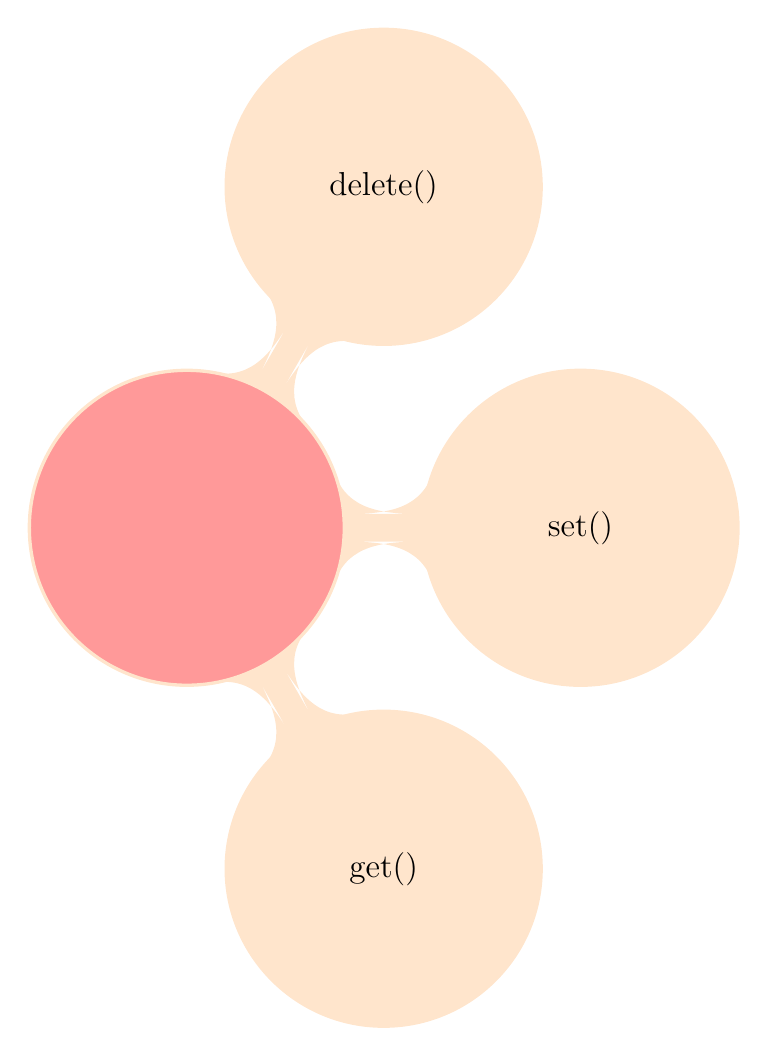
\begin{tikzpicture}[mindmap,every node/.style=concept,concept color=orange!20,grow cyclic,level 1/.style={sibling angle =60,level distance=5cm}]
\node[fill=red!40]{属性访问}
    child{node{get(访问属性)}}
    child{node{set(属性调动)}}
    child{node{delete(控制删除操作)}};

\end{tikzpicture}

\begin{python}

class Descriptor:

    def __get__(self,instance,owner):
        print('Getting:...',self,instance,owner)

    def __set__(self,instance,value):
        print('Setting...',self,instance,value)

    def __delete__(self,instance):
        print('Deleting:...',self,instance)

class Test:
	x =Descriptor()
#直接传入方法
#------------------------------------------------------------

class MyProperty:
    def __init__(self,fget=None,fset=None,fdel=None):
        self.fget=fget
        self.fset=fset
        self.fdel=fdel

    def __get__(self,instance,owner):
        return self.fget(instance)

    def __set__(self,instance,value):
        self.fset(instance,value)

    def __delete__(self,instance):
        self.fdel(instance)

class C:
    def __init__(self):
        self._x=None

    def getX(self):
        return self._x

    def setX(self,value):
        self._x=value

    def delX(self):
        del self._x

    x = MyProperty(getX,setX,delX)#传入方法

#-------------------------------------------------------------


class Celsius:
    def __init__(self,value=26.0):
        self.value=float(value)

    def __get__(self,instance,owner):
        return self.value

    def __set__(self,instance,value):
        self.value=float(value)

class Fahrenheit:
    def __get__(self,instance,owner):
        return instance.cel*1.8+32

    def __set__(self,instance,value):
        instance.cel= (float(value)-32)/1.8

class Temperature:
    cel = Celsius()
    fah = Fahrenheit()

\end{python}

\section{定制序列}
协议:\textbf{容器类型}
\begin{python}
class Countlist:
      def __init__(self,*args):#可变数量的args
            self.values=[x for x in args]
            self.count={}.fromkeys(range(len(self.values)),0)#建立字典

      def __len__(self):
            return len(self.values)

      def __getitem__(self,key):#设计访问累加
            self.count[key]+=1
            return self.values[key]
\end{python}

\section{迭代器}
iter()与next()
\begin{python}
>>> string='ss'
>>> it= iter(string)
>>> it
<str_iterator object at 0x0000000002EF64E0>
>>> next(it)         # 调取迭代器中的元素
's'
>>> next(it)
's'

>>> string ='Fishc'
>>> it= iter(string)
>>> while True:       #实现for循环
	try:
		each=next(it)
	except StopIteration:
		break
	print(each)

\end{python}

斐波那契数列
\begin{python}
class Fibs:
	def __init__(self,n=10):
		self.a=0
		self.b=1
		self.n=n
	def __iter__(self):
		return self
	def __next__(self):
		self.a,self.b=self.b,self.a+self.b
		if self.a>self.n:
			raise StopIteration
		return self.a
>>> fibs=Fibs()
>>> for each in fibs:
	print(each)

>>> fibs=Fibs(100)
>>> for each in fibs:
	print(each)

\end{python}

\section{生成器}
yield = return 可暂时执行的函数
协同程序
\begin{python}

>>> def myGen():
	print('excute')
	yield 1
	yield 2

	
>>> myG=myGen()
>>> next(myG)
excute
1
>>> next(myG)
2
>>> next(myG)
#-----------------------生成器---------------------
>>> for i in myGen():
	print(i)

>>> def fibs():
	a=0
	b=1
	while True:
		a,b=b,a+b
		yield a

		
>>> for each in fibs():
	if each >100:
		break
	print(each,end='  ')
#-------------------生成列表、字典-------------------

>>> a=[i for i in range(100) if not(i%2)and i%3]
>>> a
[2, 4, 8, 10, 14, 16, 20, 22, 26, 28, 32, 34, 38, 40, 44, 46, 50, 52, 56, 58, 62, 64, 68, 70, 74, 76, 80, 82, 86, 88, 92, 94, 98]
>>> b={i:i%2==0 for i in range(10)}
>>> b
{0: True, 1: False, 2: True, 3: False, 4: True, 5: False, 6: True, 7: False, 8: True, 9: False}
>>> c={i for i in[1,1,2,3,4,5,6,7,8,5,2,2,2]}
>>> c
{1, 2, 3, 4, 5, 6, 7, 8}
>>> e=(i for i in range(10))
>>> e
<generator object <genexpr> at 0x0000000003197C50>
>>> next(e)
0
>>> for each in e:
	print(each)
#------------------套用函数------------------------
>>> sum(i for i in range(100)if i%2)


\end{python}

\section{模块}
\tikzset{rootnode/.style={fill = blue!20,black,rectangle},node_1/.style={fill=blue!20,black,circle},node_2/.style={fill=blue!40,black,rectangle}}

\begin{tikzpicture}[->]
\node[rootnode]{模块}
  child{node[node_1](a){容器}
        child{node[node_2]{数据的封装}}}
  child{node[node_1,right=2 of a](b){函数}
        child{node[node_2]{语句的封装}}}
  child{node[node_1,right=2 of b](c){类}
        child{node[node_2]{方法与属性的封装}}};
  \draw[<->] (a)--(b);
  \draw[<->] (b)--(c);
\end{tikzpicture}

模块-->就是程序  以.py结尾
命名空间

\dirtree{%
.1 导入模块两种方法.
.2 import 模块名.
.2 from 模块名 import 函数名( * 导入所有的函数).
.2 import 模块名  as 新名字.
}

\begin{python}

    1.if __name__=='__main__':#表示当测试主程序时,则调用,作为一个模块时,不调用
            #testing->测试程序

    2.sys.path.append('C:\\路径') 添加系统模块


    3.包(package)

\end{python}

创建包(package)的做法\\

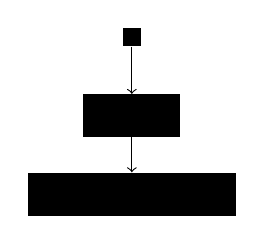
\begin{tikzpicture}

    \node[fill=blue!20,black,rectangle](a)at(0,-1){创建一个文件夹,用于存放相关的模块,文件夹的名字即包的名字};

    \node[fill=blue!30,black,rectangle](b)at(0,-2){在文件夹中创建一个——init——.py的模块文件,内容可以为空};

    \node[fill=blue!40,black,rectangle](c)at(0,-3){调用时,采用包名(package.module)};
    \draw[->](a)--(b);
    \draw[->](b)--(c);

\end{tikzpicture}

\section{标准库}
探索模块---battery\\

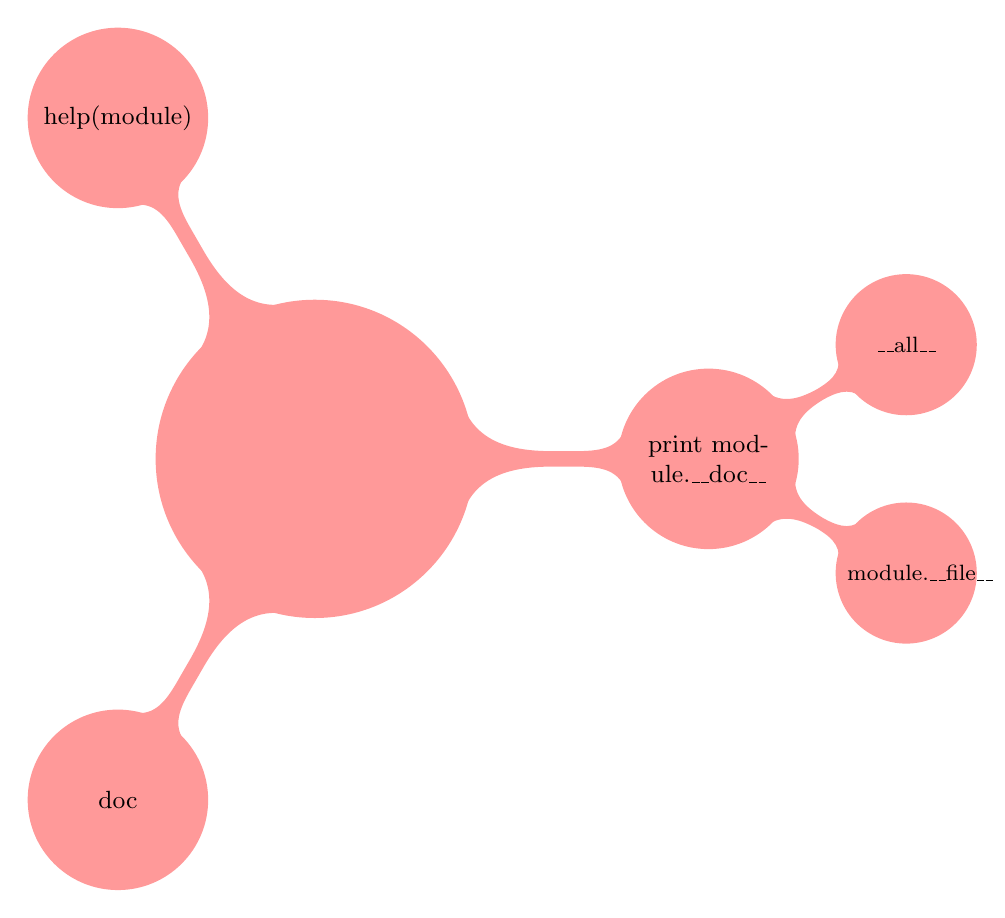
\begin{tikzpicture}[mindmap,grow cyclic,every node/.style=concept,concept color =red!40,level 1/.append style={sibling angle =120}]
  \node{寻求帮助}
    child{node{doc浏览器}
    }
    child{node{print module.\_\_doc\_\_}
        child{node{获得位置module.\_\_file\_\_}}
        child{node{\_\_all\_\_表示所有可用的接口程序}}
    }
    child{node{help(module)}
    };

\end{tikzpicture}

\section{爬虫}
web spider---网络爬虫

Uniform Resource Locator标准的资源定位表示方法\\
\dirtree{%可以出现[]()等配对符号及冒号#——\#
%$——\$
%%——\%
%{——\{
%}——\}
%~——\~{}
%\——$\backslasb$
%^——\^{}
.1 URL\newline->protocol://hostname[:por]/path/[;parameters][?query]\#frament.
.2 协议:http,https,ftp,file,ed2k.
.2 IP地址或者域名服务系统,默认端口为80.
.2 资源的具体地址,如文件名或者目录.
}

在python里一般使用urllib package
\section{实战}
\textbf{事例1——一只猫}\\

\begin{python}
import urllib.request

#urlopen 可以使字符串,也可以是object
response = urllib.request.urlopen('http://placekitten.com/2000/2000')
#<----->req =urllib.request.Request('http://placekitten.com/2000/2000')
#------->response = urllib.request.urlopen()

#读取信息
cat_img = response.read()

#获取网站信息
response.geturl()

response.info()

print(response.info())

response.getcode()

# 写入图片内容
with open('cat_2000_2000.jpg','wb') as f:
      f.write(cat_img)
\end{python}

\textbf{事例2--实现在线翻译}\\

\begin{python}

import urllib.request
import json
conntent = input('请输入需要翻译的内容:')
url ='http://fanyi.youdao.com/translate?smartresult=dict&smartresult=rule&smartresult=ugc&sessionFrom=https://www.baidu.com/link'
data = {}
data['type']='AUTO'
data['i']=conntent
data['doctype']='json'
data['xmlVersion']='1.8'
data['keyfrom']='fanyi.web'
data['ue']='UTF-8'
data['action']='FY_BY_CLICKBUTTON'
data['typoResult']='true'
data=urllib.parse.urlencode(data).encode('utf-8')

response = urllib.request.urlopen(url,data)
html =response.read().decode('utf-8')

target =json.loads(html)
print('翻译结果为:\%s'\%(target['translateResult'][0][0]['tgt']))

\end{python}

\textbf{隐藏-user-agent}\\
\dirtree{%
.1 修改headers.
.2 通过Request的headers参数修改.
.2 通过Request.add\_header()方法修改.
}

\begin{python}
import urllib.request
import json
conntent = input('请输入需要翻译的内容:')
url ='http://fanyi.youdao.com/translate?smartresult=dict&smartresult=rule&smartresult=ugc&sessionFrom=https://www.baidu.com/link'


head ={}
'''#注释-第一种方法
head['User-Agent']='Mozilla/5.0 (Windows NT 6.1; WOW64) AppleWebKit/537.36 (KHTML, like Gecko) Chrome/50.0.2661.102 Safari/537.36'
'''

data = {}
data['type']='AUTO'
data['i']=conntent
data['doctype']='json'
data['xmlVersion']='1.8'
data['keyfrom']='fanyi.web'
data['ue']='UTF-8'
data['action']='FY_BY_CLICKBUTTON'
data['typoResult']='true'
data=urllib.parse.urlencode(data).encode('utf-8')

req =urllib.request.Request(url,data,head)
#第二种方法采用
req.add_header('User-Agent','Mozilla/5.0 (Windows NT 6.1; WOW64) AppleWebKit/537.36 (KHTML, like Gecko) Chrome/50.0.2661.102 Safari/537.36')

response = urllib.request.urlopen(req)
html =response.read().decode('utf-8')


target =json.loads(html)
print('翻译结果为:%s'%(target['translateResult'][0][0]['tgt']))
\end{python}

\section{代理}
为了防止被屏蔽,可以设置搜索延迟方法一:

\begin{python}

import urllib.request
import json
import urllib.parse
import time


while True:

      content = input('请输入需要翻译的内容(输入q退出程序):')
      if content =='q':
            break


      url ='http://fanyi.youdao.com/translate?smartresult=dict&smartresult=rule&smartresult=ugc&sessionFrom=https://www.baidu.com/link'


      head ={}
      '''#注释-第一种方法
      head['User-Agent']='Mozilla/5.0 (Windows NT 6.1; WOW64) AppleWebKit/537.36 (KHTML, like Gecko) Chrome/50.0.2661.102 Safari/537.36'
      '''

      data = {}
      data['type']='AUTO'
      data['i']=content
      data['doctype']='json'
      data['xmlVersion']='1.8'
      data['keyfrom']='fanyi.web'
      data['ue']='UTF-8'
      data['action']='FY_BY_CLICKBUTTON'
      data['typoResult']='true'
      data=urllib.parse.urlencode(data).encode('utf-8')

      req =urllib.request.Request(url,data,head)
      #第二种方法采用
      req.add_header('User-Agent','Mozilla/5.0 (Windows NT 6.1; WOW64) AppleWebKit/537.36 (KHTML, like Gecko) Chrome/50.0.2661.102 Safari/537.36')

      response = urllib.request.urlopen(req)
      html =response.read().decode('utf-8')


      target =json.loads(html)
      print('翻译结果为:\%s'\%(target['translateResult'][0][0]['tgt']))

      time.sleep(5)# 等待5s


\end{python}

\textbf{代理}

步骤 如下:\\
\begin{enumerate}
  \item 参数是一个字典 {'类型':‘代理IP:端口号’}\newline
            proxy\_support =urllib.request.ProxyHandler({})
  \item 定制、创建一个opener\newline
            opener = urllib.request.build\_opener(proxy\_support)
  \item a.安装opener\newline
            urllib.request.install\_opener(opener)
  \item b.调用opener\newline
            opener.open(url)
\end{enumerate}

\textbf{IP代理地址}
\begin{python}

import urllib.request
import random
url = 'http://www.whatismyip.com.tw'
iplist =['180.76.154.5:8888','222.169.193.162:8099','222.37.6.248:80','122.67.24.136:8080']
#ip 代理网站

proxy_support = urllib.request.ProxyHandler({'http':random.choice(iplist)})

opener =urllib.request.build_opener(proxy_support)
opener.addheaders =[('User-Agent','Mozilla/5.0 (Windows NT 6.1; WOW64) AppleWebKit/537.36 (KHTML, like Gecko) Chrome/50.0.2661.102 Safari/537.36')]


urllib.request.install_opener(opener)

response =urllib.request.urlopen(url)

html = response.read().decode('utf-8')

print(html)

\end{python}

\section{抓取图片的一种方法}
\begin{python}

import urllib.request
import os
import shutil
import random
shutil.rmtree('ooxx')

def url_open(url):

      req =urllib.request.Request(url)
      req.add_header('User-Agent','Mozilla/5.0 (Windows NT 6.1; WOW64) AppleWebKit/537.36 (KHTML, like Gecko) Chrome/50.0.2661.102 Safari/537.36')
##      iplist =['124.88.67.39:80','115.231.175.68:8081']
##      proxy = random.choice(iplist)
##
##      proxy_support =urllib.request.ProxyHandler({'http':proxy})
##      opener =urllib.request.build_opener(proxy_support)
##      urllib.request.install_opener(opener)

      response = urllib.request.urlopen(url)
      html = response.read()

      print(url)

      return html



def get_page(url):
      html= url_open(url).decode('utf-8')

      a = html.find('current-comment-page')+23
      b = html.find(']',a)

      return html[a:b]


def find_imgs(url):
      html = url_open(url).decode('utf-8')
      img_addrs =[]

      a= html.find('img src=')

      while a != -1:
            b= html.find('.jpg',a,a+255)
            if b !=-1:
                  img_addrs.append('http:'+html[a+9:b+4])
            else:
                  b= a+9

            a =html.find('img src=',b)
      for each in img_addrs:
            print(each)


      return img_addrs



def save_imgs(folder,img_addrs):
      for each in img_addrs:
            filename = each.split('/')[-1]
            with open(filename,'wb') as f:
                  img = url_open(each)
                  f.write(img)




def download_mm(folder='ooxx',pages=10):
      os.mkdir(folder)
      os.chdir(folder)

      url ='http://jandan.net/ooxx/'
      page_num=int(get_page(url))

      for i in range(pages):
            page_num -=i
            page_url = url +'page-'+str(page_num)+'#comments'
            img_addrs = find_imgs(page_url)
            save_imgs(folder,img_addrs)


if __name__=='__main__':
      download_mm()

\end{python}

\section{\textbf{正则表达式}}
反斜杠可以剥夺特殊字母的特殊含义\newline
也可以赋予字符新的含义如,\ d 表示是所有数字

正则表达式:\\
\begin{python}
re.search(r'(([01]{0,1}\d{0,1}\d|2[0-4]\d|25[0-5])\.){3}([01]{0,1}\d{0,1}\d|2[0-4]\d|25[0-5])','192.168.1.1')

<_sre.SRE_Match object; span=(0, 11), match='192.168.1.1'>
# r -->源代码
# []-->字符类,搜索集合。 除了几个字符为特殊符号外,其他均当作普通字符,其中
\表示 转义 ,-表示范围,^表示放在句首 意为不匹配其中任何字符,放在中间则仅作普通符号
# [a-z1-2]-->搜索的范围表示方法两串字符之间不加任何符号
# {M,N}-->表示重复的次数M-N次
#         (M,)至少N次
#         (,N)->(0,N)
#         (N) ->匹配N次
#          * ->{0,} ->0次以上
#          + ->{1,} ->1次以上
#          ? ->{0,1}->0次或者1次

# ()-->表示分组
# .  --> 除换行符的代表任意字符
# |  --> 匹配关系正则表达式A或B
# ^ ---> 脱字符陪如果不在开始的位置,无法匹配原字符
# $ ---> 脱字符陪如果不在开始的位置,无法匹配原字符
# \. --> 剥夺  .的特殊权利
# \d --> 数字
# \D --> 匹配 非字符类
# ()\数字  -->表示引用多少次
# \A  \Z -->用于定位
# \b --> 匹配单词边界
# \B --> 匹配非单词边界
# \s -->定义空白字符; \t tab  \n 下一行  \r 空格符   \f page \v 垂直空格
# \S --> 与\s 相反
# \w --> 单词元素

#编译模型
>>> p = re.compile(r'A-z')
>>> type(p)
<class '_sre.SRE_Pattern'>
>>> p.search('i love ')
p.findall('i love')

# 编译标志
存在一个标志使得支持空格tab


\end{python}


\end{document}

%python注释快捷键ctrl+/
```

